%%%%%%%%%%%%%%%%%%%%%%%%%%%%%%%%%%%%%%%%%%%%%%%%%%%%%%%%%%%%%%%%%%%%%%%%%%%%%%%

\section{Introduction}

Equivalent sources:
The equivalent source technique has been widely used since the introduction by \citet{Dampney1969} stating any harmonic function can be approximated by the sum of discrete point source effects.

The different gridding methods, such as inverse-distance weights, polynomical fitting, spline functions (Briggs, 1974), often assume potential data are not harmonic functions. However, the total field anomaly is harmonic when the magnitude is much smaller than the magnitude of the geomagnetic field; this is true for most instances in which the total field anomaly is observed. 

Airborne data often have more data points along flight lines and much larger gaps between flight lines. The equivalent source (EQS) technique takes into account the irregularly spaced grids and the variable heights of the observed data. The EQS technique can be used for reduction to the pole, upwards continuation, modelling the lithospheric magnetic field, etc.

Taken from methodology:
Li et al. (2020) found that having an additional deeper layer of equivalent sources improved the accuracy of the predictions, particularly for the long-wavelength fields. Li et al. (2020) fit both layers to the observed data simultaneously using prisms. Due to the sensitivity matrix elements associated with the shallow layer being much larger than the elements associated with the deep layer, their method required the use of a depth-weighing factor to keep the shallow layer coefficients from dominating.

Gradient-boosted equivalent sources:

Cross validation for model selection:

Norm of the magnetic field:
The norm of the magnetic field is less dependent on the direction of magnetisation. This is particularly useful for areas with remanent magnetisation, low magnetic latitudes, sources with shallow inclination directions and sources with an unknown magnetised directions (Hidalgo-Gato, et al., 2021; Melo, et al., 2021). By calculating the norm of the magnetic anomalous field, the data is less dependent on the direction of Earth’s main field and crustal magnetisation.

Nonuniqueness

\clearpage

%%%%%%%%%%%%%%%%%%%%%%%%%%%%%%%%%%%%%%%%%%%%%%%%%%%%%%%%%%%%%%%%%%%%%%%%%%%%%%%

\section{Methodology}

The observed total field anomaly ($\Delta T$) is the difference between the measured norm of the total magnetic field ($\vec{\mathbf{T}}$) and the norm of the regional reference field ($\vec{\mathbf{F}}$, usually represented by the IGRF) at the time of measurement:
\begin{equation}
    \Delta T = \vert \vec{\mathbf{T}} \vert - \vert \vec{\mathbf{F}} \vert
    \ .
\end{equation}

\noindent
The total magnetic field ($\vec{T}$) is the sum of the anomalous magnetic field vector ($\vec{\mathbf{B}}$) and the regional field vector ($\vec{\mathbf{F}}$) \citep{Blakley1995, Langel1998, OliveiraJr2015}. The total field anomaly ($\Delta T$) can therefore be given by
\begin{equation}
    \Delta T = \vert \vec{\mathbf{F}} + \vec{\mathbf{B}} \vert - \vert \vec{\mathbf{F}} \vert
    \ .
\end{equation}
\noindent
For the majority of crustal anomalies measured by airborne and shipborne surveys, $\vec{\mathbf{B}}$ is much smaller in magnitude compared to $\vec{\mathbf{F}}$. Additionally, $\vec{\mathbf{F}}$ can be considered constant on these local to regional scales. Subsequently, $\Delta T$ can be approximated as

\begin{equation}
\label{eq:tfa_dot_product}
    \Delta T\approx  \vec{\mathbf{B}} \cdot \hat{\mathbf{F}}
    \ ,
\end{equation}

\noindent
in which $\hat{\mathbf{F}}$ is a unit vector in the same direction as the regional field. Thus, $\Delta T$ is approximately a harmonic function \citep{Blakley1995,OliveiraJr2015}.


\subsection{Equivalent Source Technique}

The equivalent source technique assumes any harmonic function \textcolor{orange}{$d(x, y, z)$} can be approximated by the sum of $M$ discrete point source effects \citep{Dampney1969, Cordell1992}:

\begin{equation}
\label{eq:eqs_technique}
\textcolor{orange}{d (x, y, z)} = \sum_{j=1}^{M} a_j(x, y, z, x'_j, y'_j , z'_j) \textcolor{teal}{c_j}
\ ,
\end{equation}

\noindent
where \textcolor{orange}{$d$} is calculated at the Cartesian coordinates ($x$, $y$, $z$) pointing in the geographic east, geographic north and upwards direction, respectively. The function $a_j(x, y, z, x'_j, y'_j , z'_j)$ is the effect of the $j$-th source with unitary physical property, located at the Cartesian coordinates $(x'_j, y'_j, z'_j)$, calculated at the observation point $(x, y, z)$. The coefficients (\textcolor{teal}{$c_j$}) represent the physical property of the $j$-th source 
(e.g. density for gravity data, magnetic moment amplitude for magnetic data).

For magnetic surveys, \textcolor{orange}{$d (x, y, z)$} from Equation~\ref{eq:eqs_technique} becomes \textcolor{orange}{$\Delta T(x, y, z)$}. The point source effects, $a_j(x, y, z, x'_j, y'_j , z'_j)$, are therefore $\vec{\mathbf{B}}_j \cdot \hat{\mathbf{F}}$ from Equation~\ref{eq:tfa_dot_product}, where $\vec{\mathbf{B}}_j$ is the magnetic field of the $j$-th dipole with unit magnetic moment ($\hat{\mathbf{m}}_j$) and is given by \citep{Blakley1995}:

\begin{equation}
    \vec{\mathbf{B}}_j (x, y, z) = C_m \dfrac{3 \left( \hat{\mathbf{m_j}} \cdot \hat{\mathbf{r_j}} \right) \hat{\mathbf{r_j}} - \hat{\mathbf{m_j}}}{{r_j}^3}
    \ .
    \label{eq:magnetic_field}
\end{equation}

\noindent
Here $C_m = \frac{\mu_0}{4 \pi} = 10^{-7} \ \text{Hm}^{-1}$ is the proportionality constant where $\mu_0$ is the magnetic permeability of free space, $\hat{\mathbf{m}}_j$ is the dipole moment unit vector and $r_j$ is the distance between the observation point and the $j$-th source:
\begin{equation}
    r_j = \sqrt{(x - x_j')^2 + (y - y_j')^2 + (z - z_j')^2}
    \ ,
\end{equation}
 

The coefficients (\textcolor{teal}{$\mathbf{c_j}$}) from Equation~\ref{eq:eqs_technique} are the norm of the magnetic moment \textcolor{teal}{$\vert \vec{\mathbf{m}}_j \vert = m_j$}. As a result, Equation~\ref{eq:eqs_technique} becomes
\begin{equation}
\label{eq:tfa_eqs}
\textcolor{orange}{\Delta T (x, y, z)} = \sum_{j=1}^{M} \left(\vec{\mathbf{B}}_j(x, y, z) \cdot \hat{\mathbf{F}}\right) \textcolor{teal}{m_j}
\ .
\end{equation}

For $N$ observation points, Equation~\ref{eq:tfa_eqs} can be arranged in a linear system which can be expressed in matrix form:

\begin{equation}
\textcolor{orange}{\begin{bmatrix}
    \Delta T_1 \\ \Delta T_2 \\ \vdots \\ \Delta T_N
\end{bmatrix}_{Nx1}} = \begin{bmatrix}
    \mathbf{B}_{11} \cdot \hat{\mathbf{F}} & \mathbf{B}_{12} \cdot \hat{\mathbf{F}} & \cdots & \mathbf{B}_{1M} \cdot \hat{\mathbf{F}} \\
    \mathbf{B}_{21} \cdot \hat{\mathbf{F}} & \mathbf{B}_{22} \cdot \hat{\mathbf{F}} & \cdots & \mathbf{B}_{2M} \cdot \hat{\mathbf{F}} \\
    \vdots & \vdots & \vdots & \vdots \\
    \mathbf{B}_{N1} \cdot \hat{\mathbf{F}} & \mathbf{B}_{N2} \cdot \hat{\mathbf{F}} & \cdots & \mathbf{B}_{NM} \cdot \hat{\mathbf{F}} \\
\end{bmatrix}_{NxM} \textcolor{teal}{\begin{bmatrix}
    m_1 \\ m_2 \\ \vdots \\ m_j
\end{bmatrix}_{Mx1}} \ ,
\end{equation}

\begin{equation}
    \textcolor{orange}{\bar{\mathbf{d}}} = \bar{\bar{\mathbf{A}}} \textcolor{teal}{\bar{\mathbf{c}}}
    \ ,
\end{equation}

\noindent
where \textcolor{orange}{$\bar{\mathbf{d}}$} is the column vector of $N$ predicted data at the observation points, \textcolor{teal}{$\bar{\mathbf{c}}$} is the column vector of $M$ coefficients (norm of the magnetic moment), and $\bar{\bar{\mathbf{A}}}$ is the $N \times M$ sensitivity (Jacobian) matrix. 


The damped least-squares solution can be obtained by minimizing the goal function, $\phi$, 

\begin{equation}
\label{eq:goal_function}
    \phi(\textcolor{teal}{\bar{\mathbf{c}}}) = \textcolor{orange}{\bar{\mathbf{r}}^T\bar{\mathbf{r}}} + \mu \textcolor{teal}{\bar{\mathbf{c}}^T\bar{\mathbf{c}}}
    \ ,
\end{equation}

\noindent
where $\theta(\textcolor{teal}{\bar{\mathbf{c}}}) = \mu \textcolor{teal}{\bar{\mathbf{c}}^T\bar{\mathbf{c}}}$ is the regularisation function, $\mu$ is the positive regularisation parameter, and $\psi(\textcolor{teal}{\bar{\mathbf{c}}}) =$ \textcolor{orange}{$\bar{\mathbf{r}}^T\bar{\mathbf{r}}$} is the data misfit function where \textcolor{orange}{$\bar{\mathbf{r}}$} is the residual between the observed and predicted data:

\begin{equation}
    \label{eqs:resdiual}
    \textcolor{orange}{\bar{\mathbf{r}}} = \textcolor{orange}{\bar{\mathbf{d}}^o} - \textcolor{orange}{\bar{\mathbf{d}}}
    \ .
\end{equation}

\noindent
Consequently, the goal function from Equation~\ref{eq:goal_function} can  be expanded to give

\begin{equation}
    \phi (\textcolor{teal}{\bar{\mathbf{c}}}) = \left(\textcolor{orange}{\bar{\mathbf{d}}^o} - \Bar{\Bar{\mathbf{A}}} \textcolor{teal}{\bar{\mathbf{c}}}\right)^T \left(\textcolor{orange}{\bar{\mathbf{d}}^o} - \Bar{\Bar{\mathbf{A}}} \textcolor{teal}{\bar{\mathbf{c}}}\right) + \mu \textcolor{teal}{\bar{\mathbf{c}}^T\bar{\mathbf{c}}}
    \ .
\end{equation}

\noindent
By minimising the goal function, the values of the source coefficients \textcolor{teal}{$\bar{\mathbf{c}}$} that best fit the observed field values can be obtained subject to the constraint. If the residual is as close as possible to zero, the observed and predicted data are very similar. Therefore, the smallest $\phi(\textcolor{teal}{\bar{\mathbf{c}}})$ gives the best fit, which can be calculated by taking the gradient of $\phi(\textcolor{teal}{\bar{\mathbf{c}}})$ and equating it to the null vector:
\begin{equation}
    \nabla_{\textcolor{teal}{\bar{c}}} \phi = 2 \Bar{\Bar{\mathbf{A}}}^T \Bar{\Bar{\mathbf{A}}} \textcolor{teal}{\Bar{\mathbf{c}}} - 2\Bar{\Bar{\mathbf{A}}}^T\textcolor{orange}{\bar{\mathbf{d}}^o} + 2\mu \textcolor{teal}{\bar{\mathbf{c}}} = \bar{\mathbf{0}}
    \ .
\end{equation}

\noindent
This can be rearranged to express the normal equation system:
\begin{equation}
    \left( \Bar{\Bar{\mathbf{A}}}^T \Bar{\Bar{\mathbf{A}}} +  \mu \bar{\bar{\mathbf{I}}} \right) \textcolor{teal}{\bar{\mathbf{c}}} = 
    \Bar{\Bar{\mathbf{A}}}^T\textcolor{orange}{\bar{\mathbf{d}}^o}
    \ ,
    \label{eq:normal_equations}
\end{equation}

\noindent
which can be solved for \textcolor{teal}{$\bar{\mathbf{c}}$}. Once \textcolor{teal}{$\bar{\mathbf{c}}$} has been estimated, Equation~\ref{eq:eqs_technique} can be used to forward model the total-field anomaly in any ($x, y, z$) location.


The norm of the anomalous magnetic field vector ($\vec{\mathbf{B}}$) caused by the $j$-th source with unit magnetic moment is given by
\begin{equation}
    \left\lvert \vec{\mathbf{B}_j}(x,y,z) \right\rvert = \sqrt{B^2_{x_j} + B^2_{y_j} +B^2_{z_j}}
    \ ,
\end{equation}

\noindent
where $B_{x_j}$, $B_{y_j}$ and $B_{z_j}$ are the three components of the anomalous magnetic field vector (Equation~\ref{eq:magnetic_field}) in the geographic easting, geographic northing and upwards direction, respectively. We can therefore adapt Equation~\ref{eq:tfa_eqs} to predict the norm of the anomalous magnetic field using the estimated dipole moment intensities (\textcolor{teal}{$\bar{\mathbf{c}}$}):
\begin{equation}
\textcolor{orange}{\left\lvert \vec{\mathbf{B}}(x,y,z) \right\rvert} = \sum_{j=1}^{M}  \left\lvert \vec{\mathbf{B}}_{j}(x,y,z) \right\rvert \textcolor{teal}{m_j}
\ .
\end{equation}


\subsection{Dual Layer Concept}

The use of two layers, a shallow one and a deep one, was first introduced by \citet{Li2020} to predict the three components of the anomalous field ($\vec{\mathbf{B}}$) from total-field anomaly observations. The deep layer was used to fit the regional magnetic field and the shallow layer was used to fit the shallow magnetic anomalies. \citet{Li2020} found that having an additional deeper layer of equivalent sources improved the accuracy of the predictions, particularly for the long‐wavelength fields. \citet{Li2020} fit both layers to the observed data simultaneously. Due to the sensitivity matrix elements associated with the shallow layer being much larger than the elements associated with the deep layer, their method required the use of a depth-weighing factor to keep the shallow layer coefficients from dominating.

Instead, here the dual layer method is modified to separate the deep and shallow sources into two different sets of parameters, \textcolor{teal}{$\bar{\mathbf{c}}^d$} and \textcolor{teal}{$\bar{\mathbf{c}}^s$}, respectively, and estimated separately. To estimate the deep layer coefficients first, the short-wavelength information has to be removed from the observed data to allow the deep layer to only capture the long-wavelength components, rather than both short- and long-wavelength components. This is achieved by block-averaging the observed line data, as described in Algorithm~\ref{alg:block_averaging}.

\begin{algorithm}[!h]
  \setstretch{1.5}
  Establish the geographic bounding box (region) of the data
  \;
  Add an amount of padding to the edges of the bounding box
  \;
  Divide the padded region into blocks of equal size
  \;
  For each block, calculate the median $(x, y, z)$ coordinates and the median data value of the observations that fall within the respective block
  \;
  \BlankLine
  \setstretch{1}
  \caption{The block averaging method.}
  \label{alg:block_averaging}
\end{algorithm}


The deep layer coefficients (\textcolor{teal}{$\bar{\mathbf{c}}^d$}) of size $M^d$, are estimated using the block-averaged data instead of the original line data with Equation~\ref{eq:normal_equations}. The deep equivalent sources are placed one beneath each block-averaged data point at a given depth. Thus, another advantage of using the block-averaged data for fitting the deep layer is the reduced computational load because of the reduced amount of data and equivalent sources in the model. The estimated dipole moments of the deep layer \textcolor{teal}{$\bar{\mathbf{c}}^d$} are then used to calculate a predicted total-field anomaly \textcolor{orange}{$\bar{\mathbf{d}}^d$} using Equation~\ref{eq:tfa_eqs} on all of the $N$ original observation points.
Subsequently, a deep layer residual vector is calculated given by
\begin{equation}
    \textcolor{orange}{\bar{\mathbf{r}}^d} = \textcolor{orange}{\bar{\mathbf{d}}^o} - \textcolor{orange}{\bar{\mathbf{d}}^d}
    \ .
    \label{eq:deep_residual}
\end{equation}

The shallow layer coefficients are estimated by fitting the $N$ deep layer residuals (\textcolor{orange}{$\bar{\mathbf{r}}^d$}). Since $N$ can be large for real-world airborne surveys (in the order of millions of observations), the fitting employs the gradient-boosted equivalent source technique from \citet{Soler2021}. As suggested by \citet{Soler2021}, the positions of the equivalent sources are calculated by block-averaging the data coordinates using a block size equal to the desired grid spacing, leading to $M^s < N$ sources. It is worth emphasizing that only the source coordinates undergo block-averaging and not the observed data themselves. Block-averaging the source coordinates reduces the computational load by reducing the number of source coefficients that need to be estimated.

Once both the coefficients for both the deep and shallow layers are estimated, the total-field anomaly can be predicted by combining the predictions of both layers:
\begin{equation}
    \label{eq:tfa_eqs_dual_layer}
  \textcolor{orange}{\Delta T (x, y, z)} = \sum_{j=1}^{M^d} \left(\vec{\mathbf{B}}^d_j(x, y, z) \cdot \hat{\mathbf{F}}\right) \textcolor{teal}{m_j^d}
  +  \sum_{j=1}^{M^s} \left(\vec{\mathbf{B}}^s_j(x, y, z) \cdot \hat{\mathbf{F}}\right) \textcolor{teal}{m_j^s}
  \ .
\end{equation}

\noindent
Likewise, the norm of the anomalous field can also be predicted by combing the predictions of both layers:

\begin{equation}
  \textcolor{orange}{\left\lvert \vec{\mathbf{B}}(x,y,z) \right\rvert} = 
  \left\lvert \sum_{j=1}^{M^d} \vec{\mathbf{B}}^d_{j}(x,y,z)\ \textcolor{teal}{m^d_j}
  +
  \sum_{j=1}^{M^s}  \vec{\mathbf{B}}^s_{j}(x,y,z)\ \textcolor{teal}{m^s_j}
  \right\rvert
  \ .
\end{equation}

A summary of this dual layer method proposed here is given in Algorithm~\ref{alg:dual_layer}.

\begin{algorithm}[!h]
  \setstretch{1.5}
  Block average the observed data
  \;
  Place $M^d$ deep equivalent sources one beneath each block-averaged data point at a given depth
  \;
  Estimate $M^d$ deep layer coefficients \textcolor{teal}{$\bar{\mathbf{c}}^d$} using the block-averaged data 
  \;
  Use the estimated dipole moments of the deep layer \textcolor{teal}{$\bar{\mathbf{c}}^d$} to predict the total-field anomaly \textcolor{orange}{$\bar{\mathbf{d}}^d$} using Equation~\ref{eq:tfa_eqs} on all of the $N$ original observation points
  \;
  Calculate a deep layer residual vector using Equation~\ref{eq:deep_residual}
  \;
  Block-average the data coordinates by a block size equal to the desired grid spacing
  \;
  Place the shallow equivalent sources beneath the newly block-averaged data coordinates
  \;
  Estimate the shallow layer coefficients \textcolor{teal}{$\bar{\mathbf{c}}^s$} by fitting the $N$ deep layer residuals \textcolor{orange}{$\bar{\mathbf{r}}^d$}
  \;
   Predict the total-field anomaly by combining the predictions of both layers using Equation~\ref{eq:tfa_eqs_dual_layer}.
  \BlankLine
  \setstretch{1}
  \caption{The dual layer equivalent source method.}
  \label{alg:dual_layer}
\end{algorithm}


\subsection{Gradient-Boosted Equivalent Sources}

Estimating \textcolor{teal}{$\bar{\mathbf{c}}$} using the damped least-squares solution (Equation~\ref{eq:normal_equations}) is computationally demanding, especially on a regional scale, due to the large number of data points. 
To overcome this problem, \citet{Soler2021} adapted the gradient-boosting method from \citet{Friedman2001}, which provides a way to fit additive models iteratively. Using this method, the shallow source coefficients (\textcolor{teal}{$\bar{\mathbf{c}}^s$}) are estimated in overlapping windows and carried out iteratively. Following \citet{Friedman2002}, \citet{Soler2021} also iterated through the windows randomly to improve the accuracy of the prediction. 
The gradient-boosted equivalent sources (GB EQS) method reduces the computational load by solving numerous smaller damped least-squares problems rather than one large problem. This method is applied to the shallow layer of equivalent sources because it is fitted to the entire dataset, which can contain millions of observations in real airborne surveys. An outline of the method is presented in Algorithm~\ref{alg:gradient_boosting}.

\clearpage
\begin{algorithm}[!h]
    \setstretch{1.5}
    Determine a set of $Q$ windows overlapping by 50\% that are equal in size and cover the whole survey area
    \;
    Shuffle the order of the windows in the set of windows
    \;
    Initialise the residuals vector with the observed data \textcolor{orange}{$\mathbf{r^1}$} = \textcolor{orange}{$\mathbf{d^o}$}
    \;
    \For{ $q = 1$ \KwTo $Q$}{
        Fit the sources inside window $q$ to the subset of residuals \textcolor{orange}{$\mathbf{r^q}$} that fall within the window to obtain the coefficient vector \textcolor{teal}{$\mathbf{c^q}$}
        \;
        Use Equation~\ref{eq:tfa_eqs} calculate a vector of predicted data \textcolor{orange}{$\mathbf{d^q}$} on all of the $N$ observation points
        \;
        Update the residuals to \textcolor{orange}{$\mathbf{r^{q+1}}$} = \textcolor{orange}{$\mathbf{r^q}$} - \textcolor{orange}{$\mathbf{d^q}$}
        \;
    }
    Predict new data values using \textcolor{orange}{$\mathbf{d}$} = $\sum\limits_{q=1}^{Q} A^q$ \textcolor{teal}{$\mathbf{c^q}$}
    \;
    \BlankLine
    \setstretch{1}
    \caption{The gradient-boosted equivalent sources method.}
    \label{alg:gradient_boosting}
\end{algorithm}

\subsection{Cross-Validation and Model Selection}

The equivalent sources model requires careful selection of appropriate values for the damping parameter, $\mu$ (see Equation~\ref{eq:goal_function}), and the depth of the equivalent sources. 
These two parameters, referred to as hyper-parameters of the inversion, significantly influence the smoothing of the model predictions. It is therefore crucial to select values for these hyper-parameters that yield accurate predictions in the unobserved locations when using the equivalent sources for interpolation. Selecting the optimal values of damping and depth requires the establishment of a metric of how well a model with a given combination of these hyper-parameters can be interpolated.

Cross-validation (CV) is a machine learning technique commonly used in statistics to obtain a metric of how successful a model is at making predictions. Data are split into two subsets: one for model training and one for model testing. This prevents overfitting by ensuring the training set is independent to the testing set. \citet{Geisser1975} introduced K-Fold CV to reduce the computational load compared to other CV methods. In K-Fold CV, data are split into K equally-sized folds. The folds 2 to $K$ are used as the training set to construct the model and the remaining fold (fold 1) is used as the testing set to validate the model \citep{Jung2017}. This is then repeated by using a subsequent fold for testing and the remaining folds for training until each fold has been used as a testing set.

\citet{Roberts2017} introduced the blocked versions of cross-validation methods for when data are spatially auto-correlated. This is necessary for when observations taken at close points tend to have similar values, which is often the case for potential-field data due to their smooth nature. In the Block K-Fold Cross-Validation (BK-CV) method, data (black dots in Figure~\ref{fig:BK-CV}) are first divided into non-overlapping spatial blocks of a specified size (orange blocks in Figure~\ref{fig:BK-CV}). These blocks are then randomly assigned to $K$ folds, ensuring each fold contains approximately the same number of data points. Data from folds 2 to $K$ are assigned to the training set (blue dots in step 1 of Figure~\ref{fig:BK-CV}), whilst the remaining fold is assigned to the testing set (red dots in step 1 of Figure~\ref{fig:BK-CV}). The training set is fitted with the equivalent source model using Equation\ref{eq:normal_equations} or the gradient-boosted equivalent sources method in order to estimate the parameters \textcolor{teal}{$\bar{\mathbf{c}}$}. The model is then used to predict \textcolor{orange}{$\mathbf{d_{test}}$}, the total field anomaly (\textcolor{orange}{$\Delta T (x, y, z)$}), on the coordinates from the testing set using Equation~\ref{eq:tfa_eqs} or the equivalent for the gradient-boosted equivalent sources.

\begin{figure}[!tb]
  \centering
  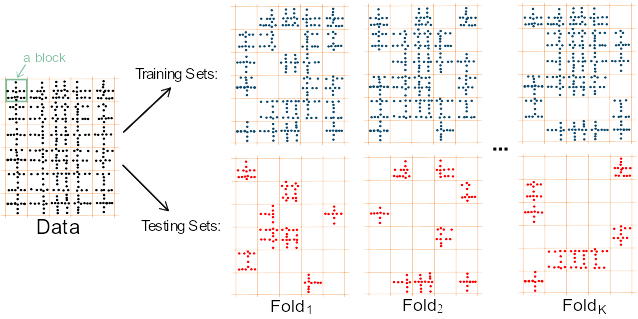
\includegraphics[width=1\linewidth]{paper/figures/bk_cv.png}
  \caption{
    The Block K-Fold Cross Validation method. The black dots are the data, the orange blocks are the non-overlapping spatial blocks of a specified size, the blue dots are the training sets for each iteration and the red dots are the testing sets for each fold.
    }
  \label{fig:BK-CV}
\end{figure}

The model accuracy can be assessed though the Root Mean Square Error (RMSE) calculated between the observed data from the testing set (\textcolor{orange}{$\mathbf{d^o_{test}}$}) and the predicted total-field anomaly also on the testing set coordinates (\textcolor{orange}{$\mathbf{d_{test}}$}):

\begin{equation}
    \label{eq:rmse}
    \text{RMSE}_k = \sqrt{\dfrac{\sum\limits_{i=1}^L \left(\textcolor{orange}{{d^o_{test_i}}} - \textcolor{orange}{{d_{test_i}}}\right)^2}{L}}
    \ ,
\end{equation}

\noindent
for $L$ number of testing points. This BK-CV process is iterated until all the folds have been used for both testing and training (see Figure~\ref{fig:BK-CV}). The overall BK-CV RMSE is determined by taking the average of all the $\text{RMSE}_k$ values across the folds. This BK-CV is summarised in Algorithm~\ref{alg:BK-CV}.

\begin{algorithm}[!h]
    \setstretch{1.5}
    Split the data into blocks of a given size
    \;
    Split the blocks randomly into K folds, with roughly the same number of data points per fold
    \;
    \For{each fold $k$}{
        Assign fold $k$ to the testing set and the remaining folds to the training set
        \;
        Estimate the parameters \textcolor{teal}{$\bar{\mathbf{c}}_k$} using the data from the training set and Equation~\ref{eq:normal_equations} or the gradient-boosted equivalent sources method
        \;
        Predict the total-field anomaly \textcolor{orange}{$\Delta T (x, y, z)$} on the coordinates of the testing set using Equation~\ref{eq:tfa_eqs}
        \;
        Calculate the $\text{RMSE}_k$ between the observed data from the testing set (\textcolor{orange}{$\mathbf{d^{o}_{test}}$}) and the predicted total-field anomaly (\textcolor{orange}{$\mathbf{d_{test}}$}) using Equation~\ref{eq:rmse}
        \;
    }
    Calculate the BK-CV RMSE by taking the average of all the $\text{RMSE}_k$ calculated for each fold.
    \BlankLine
    \setstretch{1}
    \caption{The Block K-fold Cross-Validation method.}
    \label{alg:BK-CV}
\end{algorithm}

To determine the optimal hyper-parameters for each layer, a range of values for damping and depth is systematically generated. \citet{Dampney1969} suggests bounds of 2.5 to 6 times the average distance to the nearest neighboring data points for the depth of equivalent sources. This range is utilised for the deep equivalent sources to ensure the regional long-wavelength signals are captured. For the shallow layer, a range of depths between the data heights and the deep layer are employed. Additionally, a range of $1 \times 10^{-10} \text{ to } 1 \times 10^{10}$ is used for the damping parameter $\mu$ (see Equation~\ref{eq:goal_function}). Once these ranges are defined, a comprehensive set of all the possible combinations of these hyper-parameters is created. For each combination, the BK-CV method (Algorithm~\ref{alg:BK-CV}) is employed to determine the corresponding BK-CV RMSE, which serves as the performance metric. The combination that yields the smallest BK-CV RMSE is then selected as the optimal set of parameters for the final equivalent source model.


%%%%%%%%%%%%%%%%%%%%%%%%%%%%%%%%%%%%%%%%%%%%%%%%%%%%%%%%%%%%%%%%%%%%%%%%%%%%%%%
\section{Synthetic Data Application}

To assess the accuracy of the interpolations, the method was applied to synthetic datasets containing magnetic sources with varying shapes, sizes, depths and induced magnetisations. The synthetic dataset for this paper utilises the coordinates from the ICEGRAV 2013 aeromagnetic dataset \citep{ICEGRAV_data}, as detailed in Section~\ref{sec:real_application}. These coordinates were projected using the Universal Polar Stereographic (UPS) projection, specifically for the South Pole region. The Earth's main magnetic field direction was set to match the orientation at the time of the original measurements, with an inclination of -65$^\circ$ and declination of 35$^\circ$, consistent with the real aeromagnetic dataset. The regional magnetic field was modelled on a regularly spaced grid covering the entire survey area, located at 60km beneath the surface with an oscillating height of 15 km amplitude. The magnetisation for the regional field was specified to have an inclination of -50$^\circ$, declination of 40$^\circ$ and magnitude of $5 \cdot 10^{12}$nT. Pseudo-random Gaussian noise, with a standard deviation of 5nT, was also applied to the regional field. Additionally, a regional dipole was added to study the effects of a truncating regional signal (see Section~\ref{sec:truncated_regional} for further details). This dipole was placed at coordinates [2250km, 2730km, -70km], with a magnetisation of 55$^\circ$ inclination, 45$^\circ$ declination and $2 \cdot 10^{13}$nT magnitude. The descriptions of the shallower synthetic sources can be found in Table~\ref{table:shallow_sources}, in which the characteristics of their shape, location and magnetisation is outlined.
\clearpage
\begin{table}[hbt!]
\centering
\begin{tabular}{c c c c c c}
\hline
Source & Shape & Location (km) &  & Magnitisation & \\
\cline{4-6}
 &  &  & Inclination ($^\circ$) & declination ($^\circ$) & Magnitude (nT) \\
\hline
1 & Oval & [1930, 3030, -6] & 75 & 60 & $2 \cdot 10^{10}$ \\
2 & Irregular & [1960, 2980, -0.8] & -60 & 45 & $3 \cdot 10^{9}$ \\
3 & Small Dipole & [1950, 2785, -0.5] & 45 & -65 & $5 \cdot 10^{10}$ \\
4 & Small Dipole	& [2100, 3011, -0.5] & 45 & -65 & $5 \cdot 10^{10}$ \\
5 & Small Dipole & [2110, 2955, -0.5] & 45 & -65 & $5 \cdot 10^{10}$ \\
6 & Small Dipole & [2150, 2750, -0.5] & 45 & -65 & $5 \cdot 10^{10}$ \\
7 &	Linear (Dyke) & [2200, 2950, -1] & -70 & 80 & $1 \cdot 10^{9}$ \\
8 & Linear (Dyke) & [2220, 2870, -5] & -70 & 80 & $2 \cdot 10^{9}$ \\
9 & Irregular & [2230, 2820, -0.9] & 50 & 70 & $5 \cdot 10^{9}$ \\
10 & Large Dipole & [2260, 2830, -8] & -70 & 40 & $1 \cdot 10^{10}$ \\
\hline
\end{tabular}
\caption{Descriptions of the shallower synthetic sources.}
\label{table:shallow_sources}
\end{table}

\subsection{With and without dual layer}
To assess the performance of a single verse dual layer of equivalent sources, the single layer of equivalent sources was first applied using the gradient-boosted equivalent sources (GB EQS) method (see Algorithm~\ref{alg:gradient_boosting}). To ensure optimal selection of the hyper-parameters, the Block K-Fold Cross-Validation (BK-CV) method (see Algorithm~\ref{alg:BK-CV}) was employed, using a block size of 30 km $\times$30 km over a wide range of parameter values. The optimal hyper-parameters, which resulted in the lowest BK-CV RMSE, were a damping value of $1 \cdot 10^{2}$ and a relative depth of 35km. With these optimised parameters, the GB EQS method (see Algorithm~\ref{alg:gradient_boosting}) was applied using a window size of 250 km $\times$ 250 km. To minimise errors in the initially selected windows of the iteration, the method was repeated twice. 

The resulting predictions for the total field anomaly along the survey lines, the regularly gridded lines, and the norm of the magnetic field along the regularly gridded lines are shown in Figure~\ref{fig:single_layer_synthetic}. The prediction of the total field anomaly along the survey lines (Figure~\ref{fig:single_layer_synthetic}b) provides overall an accurate prediction, with an RMSE of 8.5nT. However, it underestimates the magnitude of the four small, shallow dipoles, a pattern consistent with the predictions for both, the total field anomaly (Figure~\ref{fig:single_layer_synthetic}e) and the norm of the magnetic field (Figure~\ref{fig:single_layer_synthetic}h) on a regular grid. Furthermore, the single layer model introduces undulating ripple effects at the edges of the sources, especially along the dykes. It also generates edges effects at the borders of the survey area. These results highlight a key challenge when fitting both, the long-wavelength components and the short-wavelength components simultaneously with a single layer.

Further exploration of the single layer model reveals an inherent trade-off: when placing the equivalent source layer deeper, it captures the regional, long-wavelength signals more effectively but struggles with the short-wavelength signals. Conversely, placing the equivalent source layer shallower, improves the capture of the short-wavelength signals but compromises the ability to determine the regional, long-wavelength signals. This balancing act emphasises the limitations of using a single layer approach in modelling multi-scale sources and underlines the need for using a multi-layer model.
\clearpage

\begin{figure}[!h]
\centering
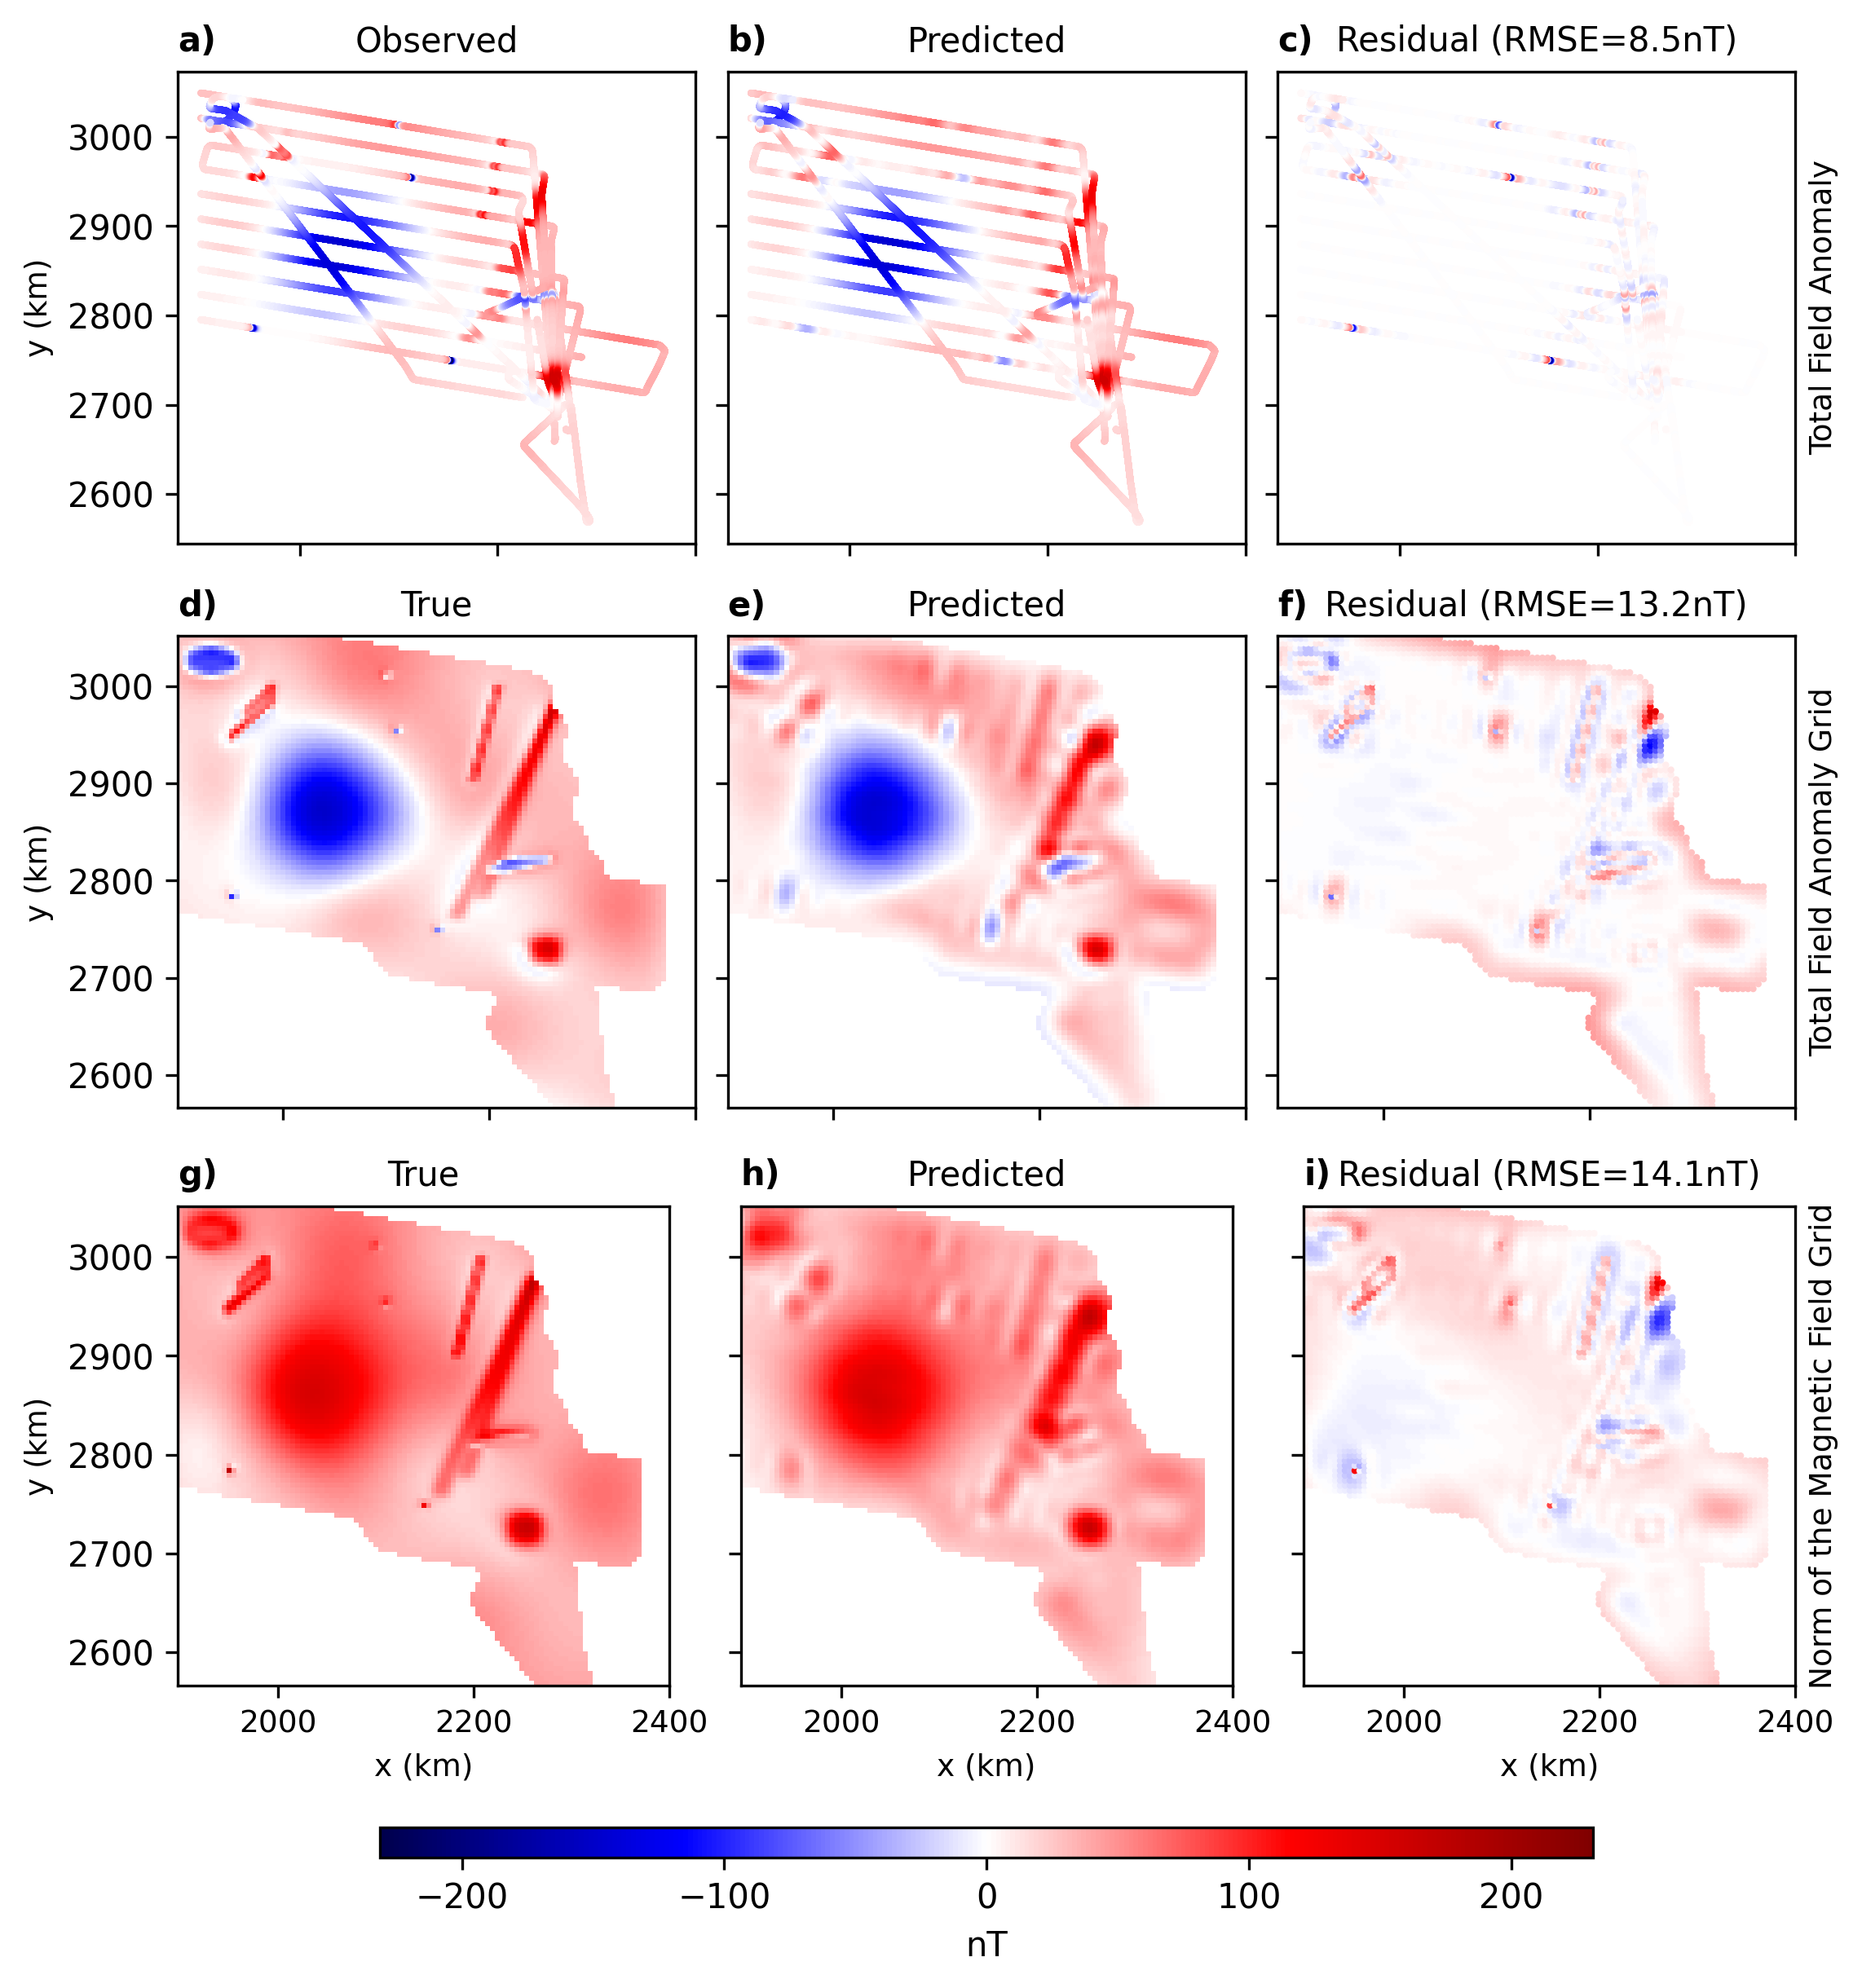
\includegraphics[width=1\linewidth]{figures/single_layer_synthetic.png}
\caption{
    INSERT CAPTION
}
\label{fig:single_layer_synthetic}
\end{figure}

To explore the potential benefits of a dual layer model, the dual layer equivalent source method (see Algorithm~\ref{alg:dual_layer}) was applied. The observed data was block averaged using different block spacings in order to determine the ideal size that isolates the long-wavelength signals for the deep layer to fit. When the block spacing is too small, some of the short-wavelength signals are captured, resulting in the deep layer not capturing all of the regional, long-wavelength signals due to trying to fit both long- and short-wavelengths. When the block spacing is too large, not all of the regional signals are captured either. Those chosen ideal block spacing for this synthetic data was 25 km $\times$ 25 km with a padding of $0.2 \times $ block spacing. The use of padding allows for more data points that fall along the survey boundary to be used, reducing the potential for edge effects at the borders that were seen in the single layer model. Using the BK-CV method (see Algorithm~\ref{alg:BK-CV}) with a block size of 100 km $\times$ 100 km, the optimal hyper-parameters for the deep layer, which resulted in the lowest BK-CV RMSE, were a damping value of 1 and a relative depth of approximately 117 km ($6 \cdot $ grid spacing). The shallow layer was then fitted to the residuals from the deep layer in order to focus on fitting the shorter-wavelength signals, as well as correct potential errors caused by the deep layer. The GB EQS method (see Algorithm~\ref{alg:gradient_boosting}) was utilised with a window size of 250 km $\times$ 250 km, matching the single layer model. To optimise the shallow layer’s hyper-parameters, the BK-CV method was applied with a block size of 30 km $\times$ 30 km (the same as the single layer model) to account for local variations in the data. The optimal hyper-parameters for the shallow layer, resulting in the lowest BK-CV RMSE, were a damping value of $1 \cdot 10^{2}$ and a relative depth of 17 km. The GB EQS method (see Algorithm~\ref{alg:gradient_boosting}) was applied twice to the shallow layer to minimise potential errors in the initial windows selected in the iteration, similar to the single layer model. 

The results for the total field anomaly along the survey lines, regularly gridded lines, and the norm of the magnetic field on the regularly gridded lines are shown in Figure~\ref{fig:dual_layer_synthetic}. The dual layer model provides a significantly improved prediction of the total field anomaly along the survey lines (Figure~\ref{fig:dual_layer_synthetic} b), with an RMSE of 4.7nT, particularly in capturing the four small dipoles. It also demonstrates the method is able to interpolate onto regularly gridded lines and upward continue to a constant height (see Figure~\ref{fig:dual_layer_synthetic} e and h). Additionally, the regional field prediction is much smoother, with no edge effects at the survey borders or along the dykes. The dual layer model successfully reduces the undulating ripple effects near the edges of the sources. However, the dual-layer method does face challenges when predicting on the regular grid (Figure~\ref{fig:dual_layer_synthetic} e and h). Specifically, the method struggles with artifacts related to the flight lines, particularly along the dykes. The gaps between the survey lines appear more pronounced in these areas, leading to visible discontinuities. This issue could be addressed by adjusting the depth of the shallow layer, but in doing so may impact the accuracy of the small anomalies such as the small dipoles.
\clearpage

\begin{figure}[!h]
\centering
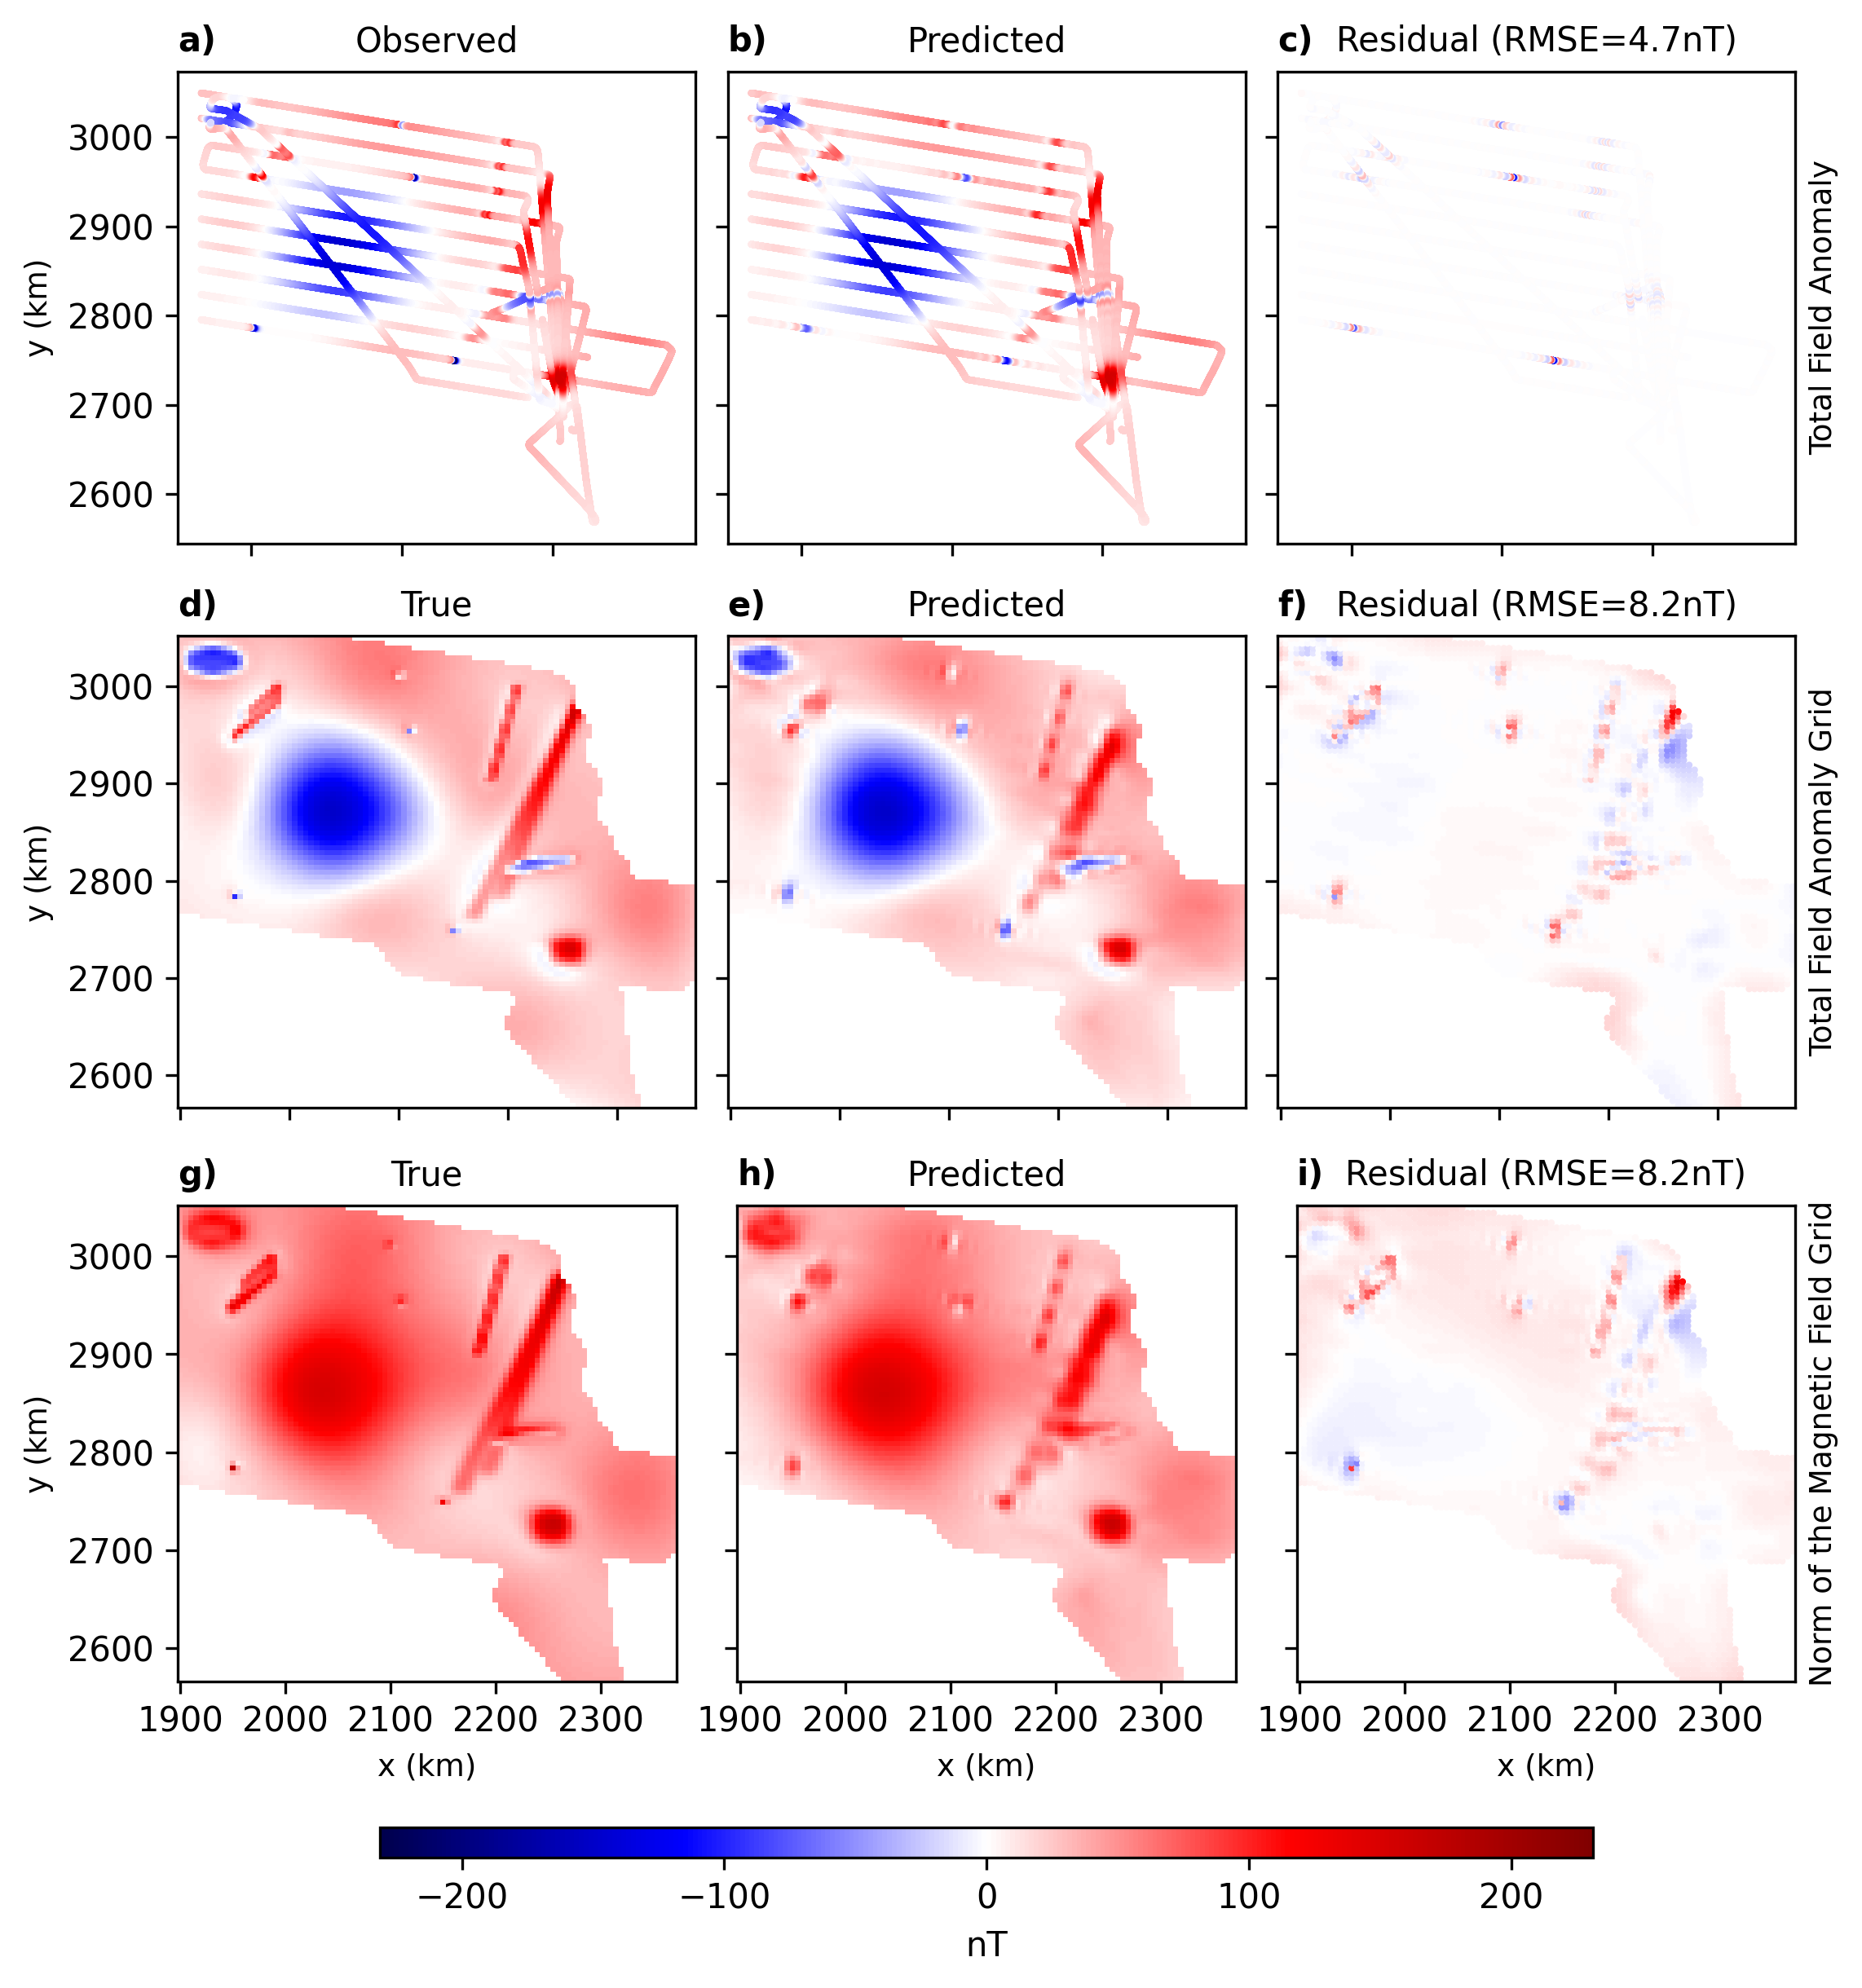
\includegraphics[width=1\linewidth]{figures/dual_layer_synthetic.png}
\caption{
    INSERT CAPTION
}
\label{fig:dual_layer_synthetic}
\end{figure}
\

Overall, the dual layer approach improves predictions by allowing the deep layer to capture the regional, long-wavelength signals, whilst the shallow layer focuses on the short-wavelength signals and corrects potential errors from the deep layer. This combination enhances the accuracy when compared to the single layer approach, illustrating the advantages of using multiple layers of equivalent sources to model multi-scale sources. Applying padding to the deep layer reduces the edge effects along the survey borders, a common artefact when using a single layer model. The BK-CV method provides a more automated and efficient way to select optimal hyper-parameters. Additionally, the use of the GB EQS method reduces the computational load and the processing time. By repeating this method twice also helps to minimise errors in the initial selection of windows during the iteration.


\subsection{Truncated Regional}
\label{sec:truncated_regional}
The impact of a truncated regional signal was also investigated after observing the single layer approach struggles to accurately predict the regional field. To assess this effect, both the single and dual layer models were applied while progressively truncating the regional dipole by moving it beyond the survey boundary. As the regional dipole became increasingly truncated, the RMSE for both models increased, particularly for the prediction of the norm of the magnetic field. However, the dual layer approach consistently exhibited a lower RMSE compared to the single layer approach, suggesting it provides more reliable predictions in the presence of a truncated regional field signal. Furthermore, the single layer approach was more susceptible to edge effects as the regional dipole was moved further out of the survey bounds. On the contrary, the dual layer approach mitigated these edge effects, further highlighting the importance of using a multi-layer approach.

%%%%%%%%%%%%%%%%%%%%%%%%%%%%%%%%%%%%%%%%%%%%%%%%%%%%%%%%%%%%%%%%%%%%%%%%%%%%%%%
\section{Real Data Application}
\label{sec:real_application}

The method was applied to the open-access aeromagnetic survey data from the ICEGRAV campaigns \citep{ICEGRAV_data}, which spanned from 2010 to 2013. The data covers parts of interior East Antarctica and the Antarctic Peninsula, including key areas such as the Dronning Maud Land ice stream systems and the Recovery Lakes drainage basin. This dataset was selected to showcase the effectiveness of the method on real-world data that features irregular survey flight lines, substantial spacing between those lines and varying line altitudes. The dataset’s distinctive characteristics, in terms of its vast geographical coverage, complex data collection and large amount of data points (404,363 data points), provide a robust and challenging test case for evaluating the method's performance in complex conditions.

The coordinates of this dataset were first projected using the Universal Polar Stereographic (UPS) projection, specifically for the South Pole region. The dual layer equivalent source method (see Algorithm~\ref{alg:dual_layer}) could then be applied to the observed data, which has already undergone preprocessing \citep{ICEGRAV_data}. To fit the deep equivalent source layer, the observed data was block-averaged using different block spacings to determine the ideal size for isolating most of the long-wavelength signals. A block spacing of 15 km $\times$ 15 km, with a padding of $ 0.3 \times $ the block spacing, was selected. The padding allows for additional data points along the survey boundary, reducing the potential for edge effects at the borders. The BK-CV method (see Algorithm~\ref{alg:BK-CV}) was applied with a block size of 200 km $\times$ 200 km to determine the optimal hyper-parameters which yield the lowest BK-CV RMSE. The chosen parameters were a damping value of 10 and a relative depth of approximately 55 km. The shallow layer was then fitted to the residuals from the deep layer using the GB EQS method (see Algorithm~\ref{alg:gradient_boosting}) with a window size of 400 km $\times$ 400 km. The BK-CV method (see Algorithm~\ref{alg:BK-CV}) was utilised again to determine the optimal hyper-parameters for the shallow layer. Using a block size of 20 km $\times$ 20 km, the chosen parameters with the lowest BK-CV RMSE were a damping value of 100 and a relative depth of approximately 10 km. The GB EQS method (see Algorithm~\ref{alg:gradient_boosting}) was applied twice to the shallow layer to minimise potential errors in the initially selected windows of the iterations.

The results for the total field anomaly along the survey lines are shown in Figure~\ref{fig:real_line_pred}. The dual layer provides a good prediction of the complicated dataset, with an RMSE of 27.3nT.

\begin{figure}[!h]
\centering
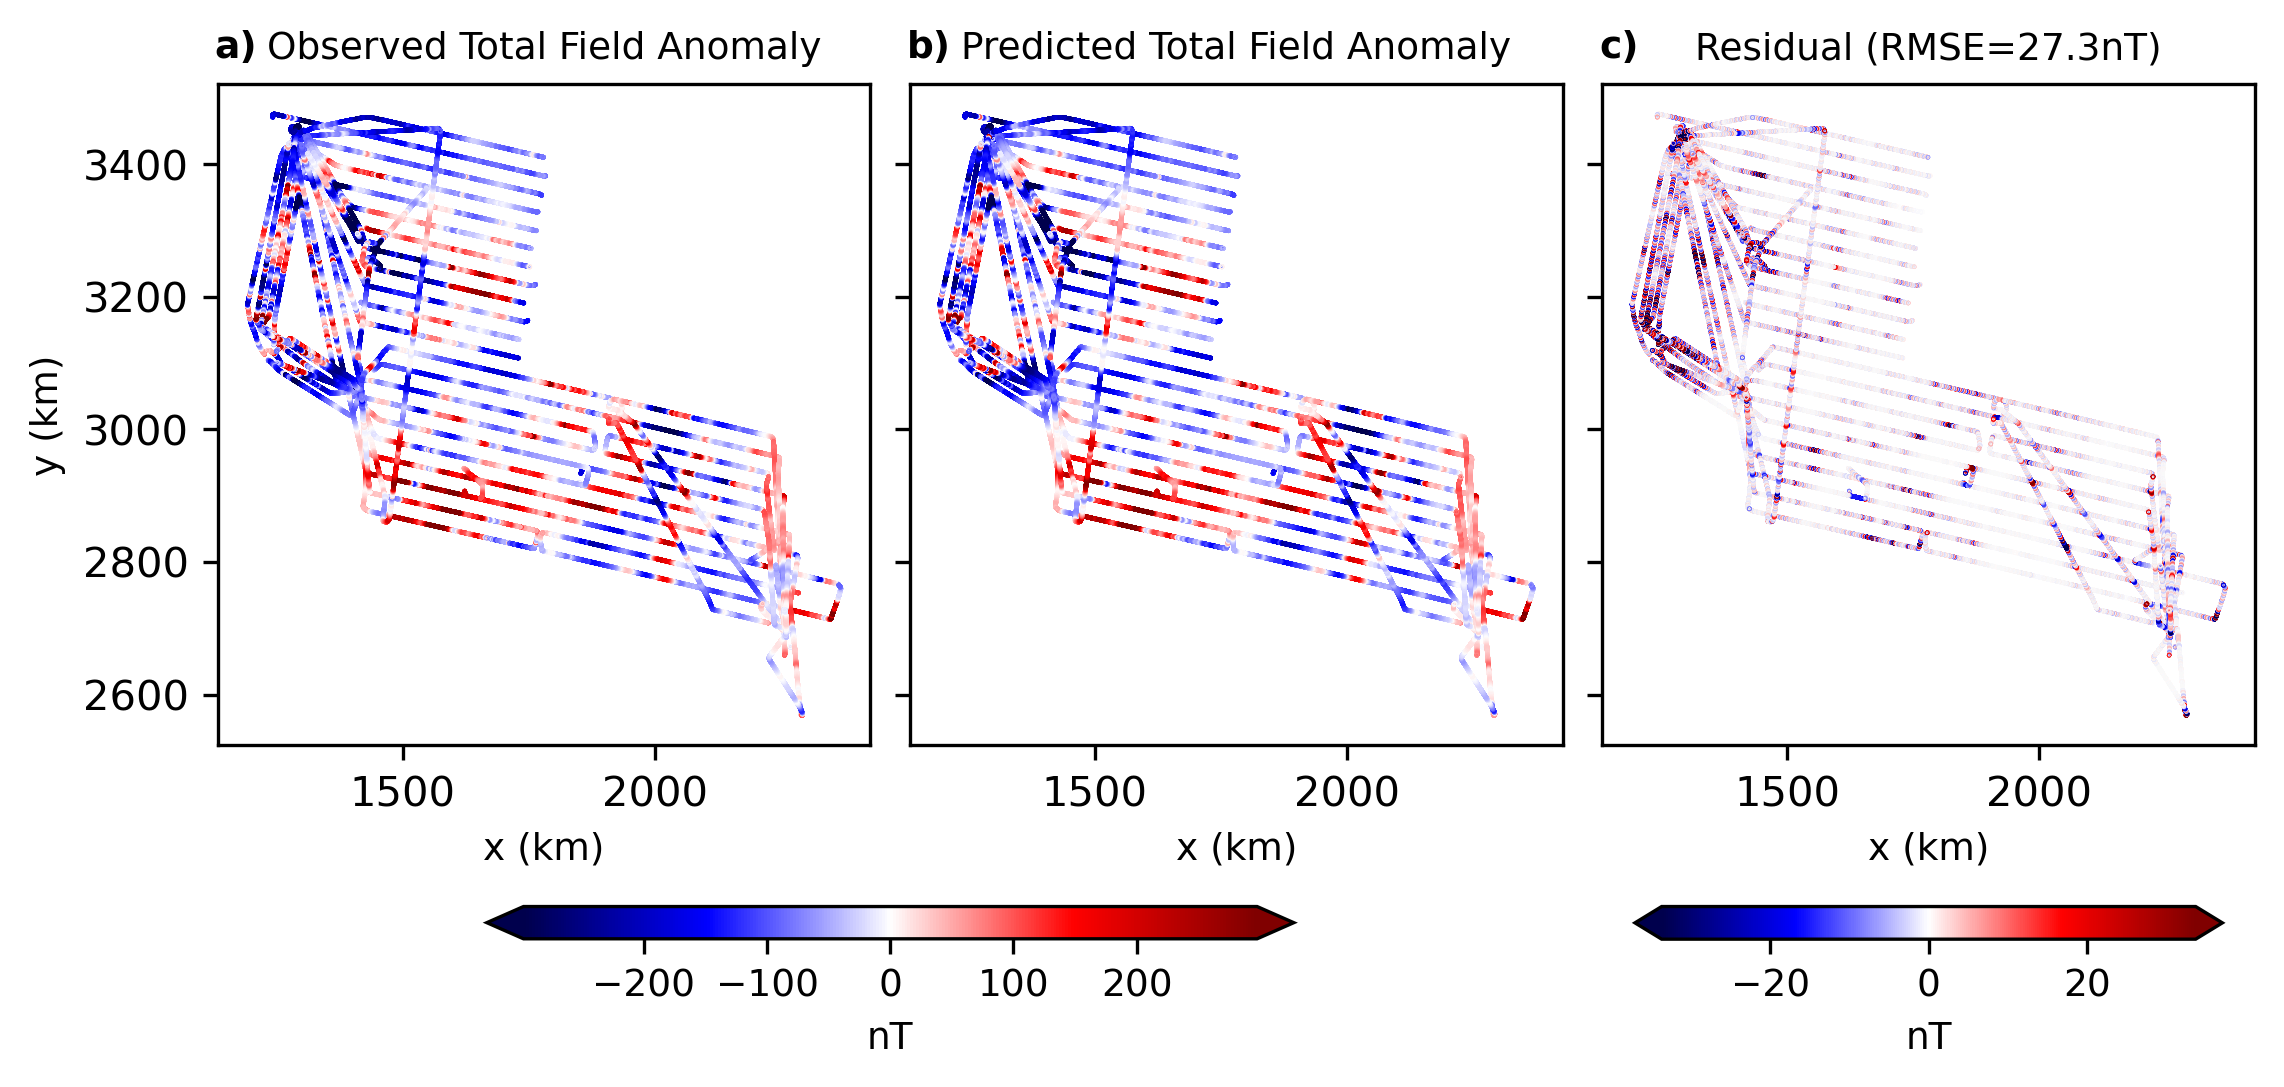
\includegraphics[width=1\linewidth]{paper/figures/real_line_pred.png}
\caption{
    INSERT CAPTION
}
\label{fig:real_line_pred}
\end{figure}

The predictions of the total field anomaly and norm of the magnetic field on a regular grid are shown in Figure~\ref{fig:real_grid_pred}. Here, the method demonstrates its ability to interpolate onto regularly gridded lines, as well as upward continue to a constant height. The grid predictions reveal numerous points with magnetidue close to 0nT, a pattern that is also present in the observed data. However, it remains uncertain whether these near-zero values represent real values or if they are artifacts introduced during the data preprocessing. If the latter is the case, more careful preprocessing is necessary before applying the equivalent source method.

\begin{figure}[!h]
\centering
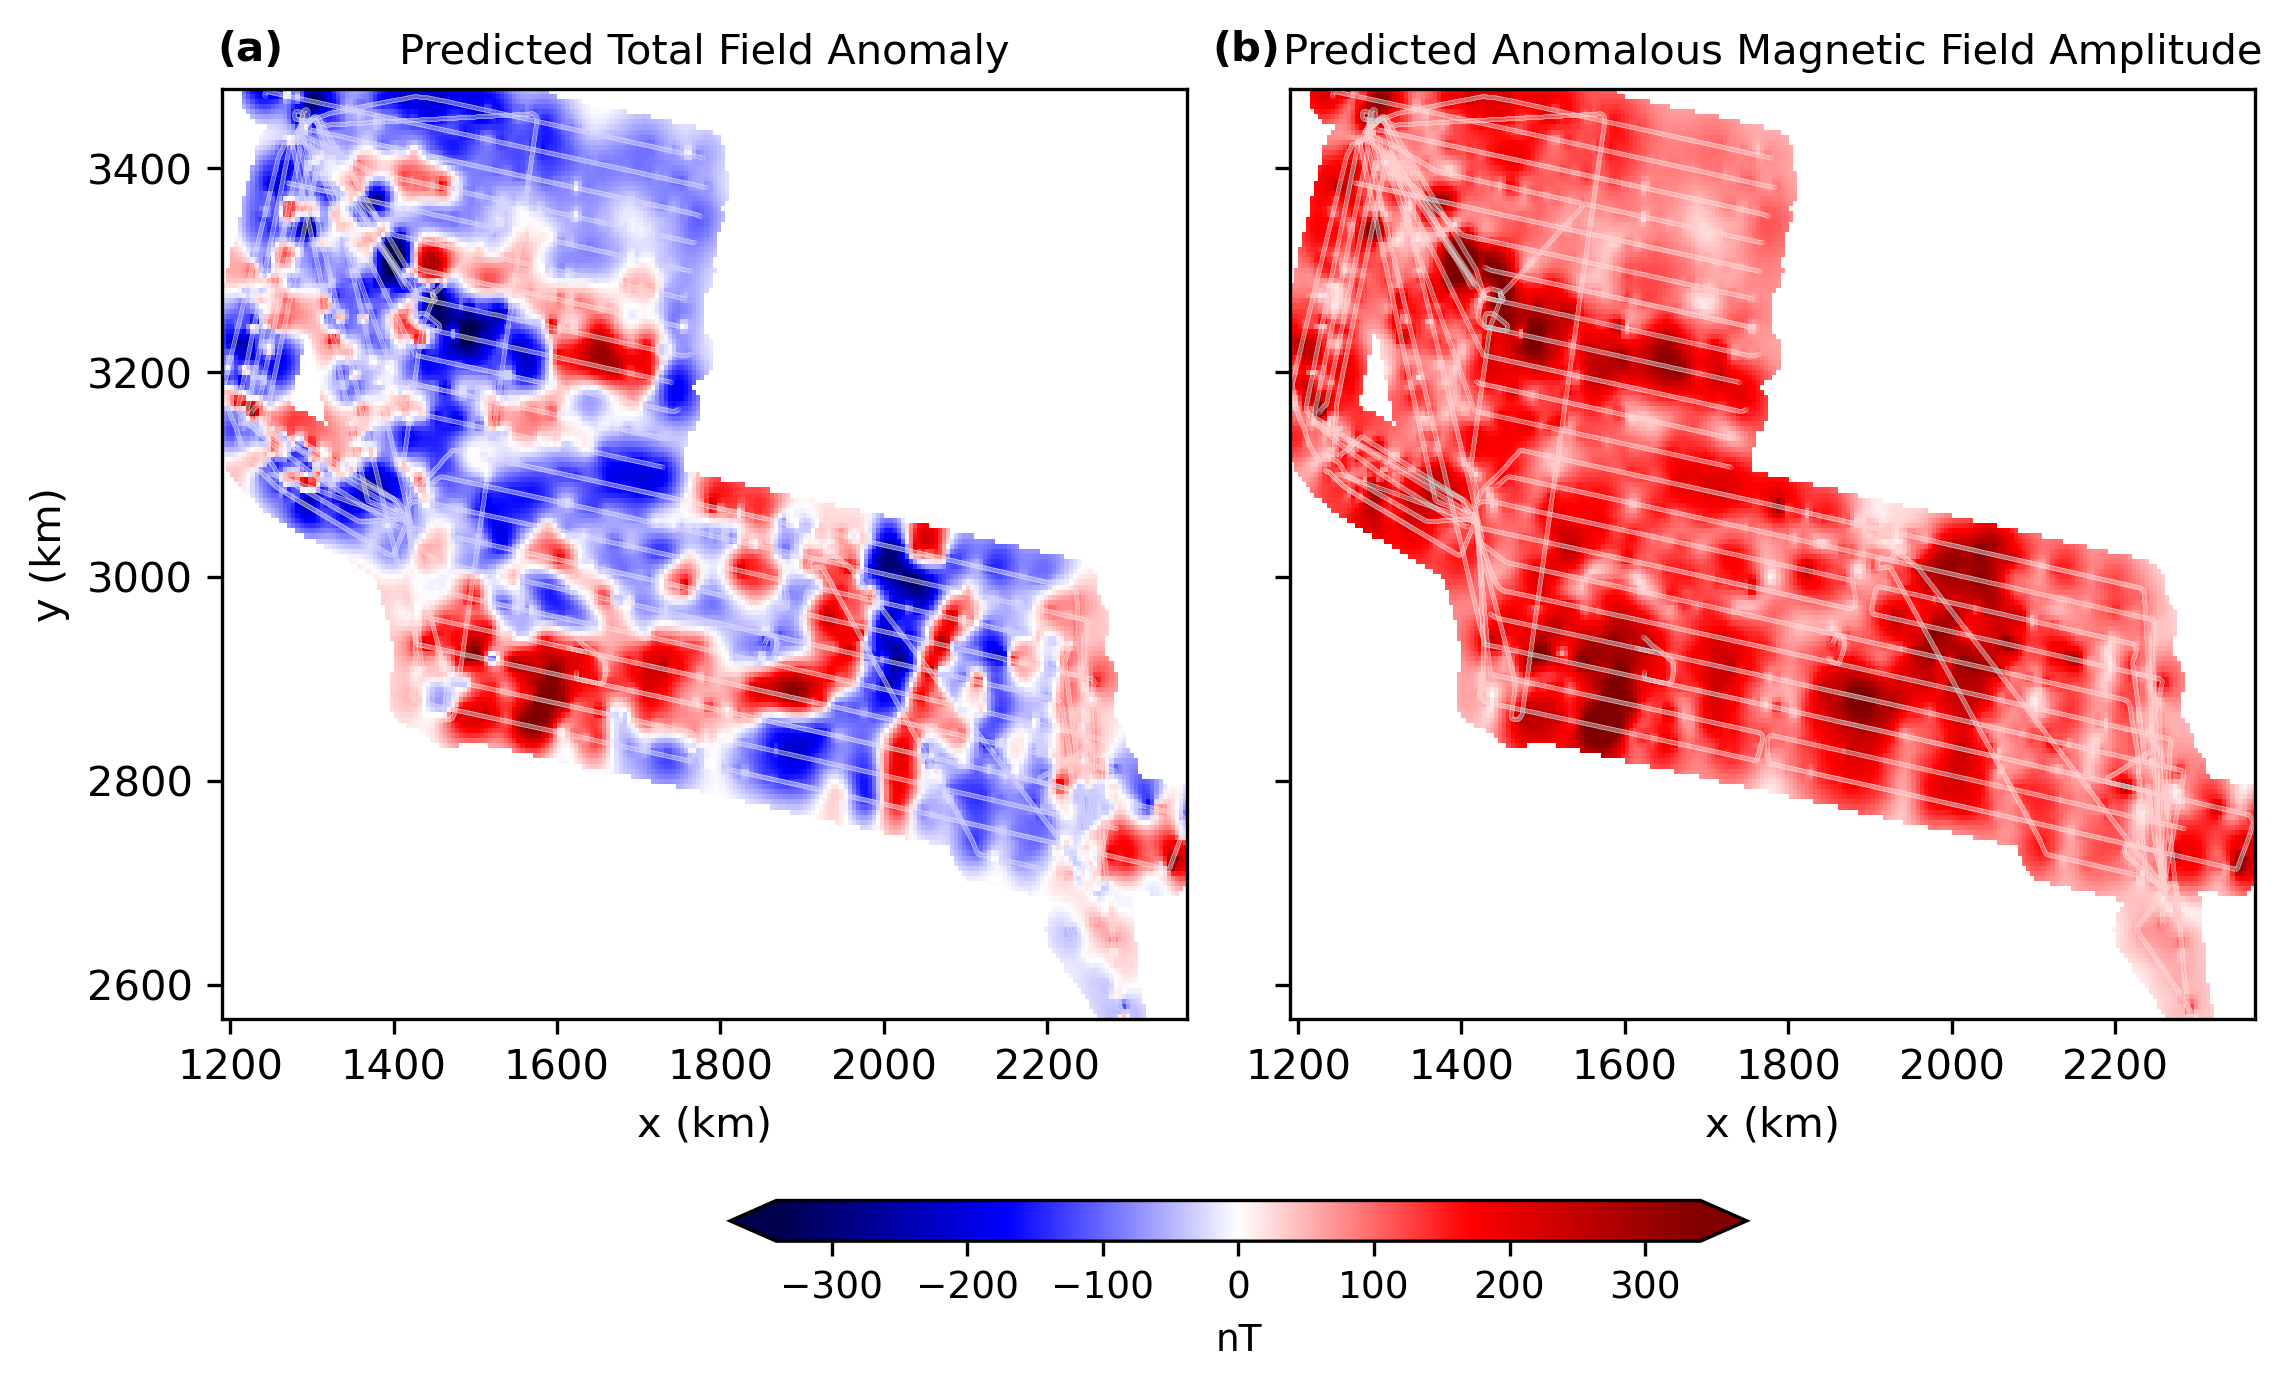
\includegraphics[width=1\linewidth]{paper/figures/real_grid_pred.png}
\caption{
    INSERT CAPTION
}
\label{fig:real_grid_pred}
\end{figure}
\clearpage

%%%%%%%%%%%%%%%%%%%%%%%%%%%%%%%%%%%%%%%%%%%%%%%%%%%%%%%%%%%%%%%%%%%%%%%%%%%%%%%
\section{Conclusion}

\lipsum[1]


%%%%%%%%%%%%%%%%%%%%%%%%%%%%%%%%%%%%%%%%%%%%%%%%%%%%%%%%%%%%%%%%%%%%%%%%%%%%%%%
\section{Open research}

The Python source code used to produce all results and figures presented here
is available at \url{https://github.com/\GitHubRepository} and
\url{https://doi.org/\ArchiveDOI} under the MIT open-source license.

Here we should cite all of the main software used, like Jupyter, numpy, scipy,
matplotlib, Fatiando, etc.

Cite any data sources as well.

%%%%%%%%%%%%%%%%%%%%%%%%%%%%%%%%%%%%%%%%%%%%%%%%%%%%%%%%%%%%%%%%%%%%%%%%%%%%%%%
\section{Acknowledgements}

We are indebted to the developers and maintainers of the open-source software
without which this work would not have been possible.
Acknowledge any non-author contributors to this study.
Statement about funding.

% Thank the editors and reviewers after review.
